% Note when we get to this section we can introduce temporal variation by stretching or shrinking our signals to augment our dataset to get more samples (and simulate potential an older adult).

\section{Selecting Cooking Tasks}
To employ some of the time-series classification methods discussed in Chapter \ref{chp:ts-classification}, a dataset of the proposed positional + IMU system is required. Chapter \ref{chp:lit-review}'s section on the traditional assessments of ADLs will serve as a basis for the selection of tasks to perform and collect data from. Of the assessments discussed, Table \ref{tab:cooking-task-summary} summarizes the assessments with cooking tasks mentioned in its procedure.

\begin{table}[ht]
    \small
    \centering
    \caption{Cooking tasks in the Assessment tools for the IADLs.}
    \label{tab:cooking-task-summary}
    \renewcommand{\arraystretch}{1.5}
    \begin{tabularx}{\textwidth}{>{\hsize=.8\hsize}X X }
        \hline
        \textbf{Tool} & \textbf{Tasks} \\
        \hline
        PASS & making soup with water/milk \\
        & making muffins in the oven \\
        & cutting up fruit \\
        Self-Assessment PD Disability Scale & making a cup of tea \\
        & inserting electrical plug \\
        & pouring milk from bottle \\
        & opening tins \\
        & washing \\
        Melbourne Low-vision ADL Index & preparing meals \\
        Lawton Instrumental ADL Scale & plans, prepares and serves adequate meals independently \\
        Frenchay Activities Index & preparing main meals \\
        Texas Functional Living Scale & Describe how to make peanut butter and jelly sandwich \\
        \hline
    \end{tabularx}
\end{table}

Of the assessments in Table \ref{tab:cooking-task-summary}, the cooking task(s) in the Melbourne Low-vision ADL Index, Lawton Instrumental ADL Scale, Frenchay Activities Index, and Self-Assessment PD Disability Scale are all questionnaires and as a result do not have concrete steps on how the task should be performed. Futhermore, the Melbourne Low-vision ADL Index, Lawnton Instrumental ADL Scale and the Frenchay Activities Index only have general requirements for the cooking task such as the ability to "prepare meals," and "plans, prepares and serves adequate meals independently." These general cooking tasks may be useful in the evaluation of ADL ability in a questionnaire format by requesting the older adult to holistically consider their ability to cook, but may not be the best candidates when looking for fine-grained actions to extract. 

The remaining 2 assessment tools, the Texas Functional Living Scale and Performance Assessment of Self-Care Skills (PASS), mention cooking task(s) that requires a clinician to evaluate. Upon closer inspection of the Texas Functional Living Scale, however, the individual is only required to describe the task and not actually perform it. The only candidate that has clear cooking tasks broken down into their fine-grained actions is the PASS and will be used as a reference for the experiment protocol and extraction of fine-grained tasks. 3 Cooking Scenarios are presented in the PASS: making soup with water/milk, making muffins in the oven, and cutting up fruit. The 3 cooking scenarios are shown in Figures \ref{fig:PASS-soup}-\ref{fig:PASS-muffin}.


\begin{figure}[ht]
    \centering
    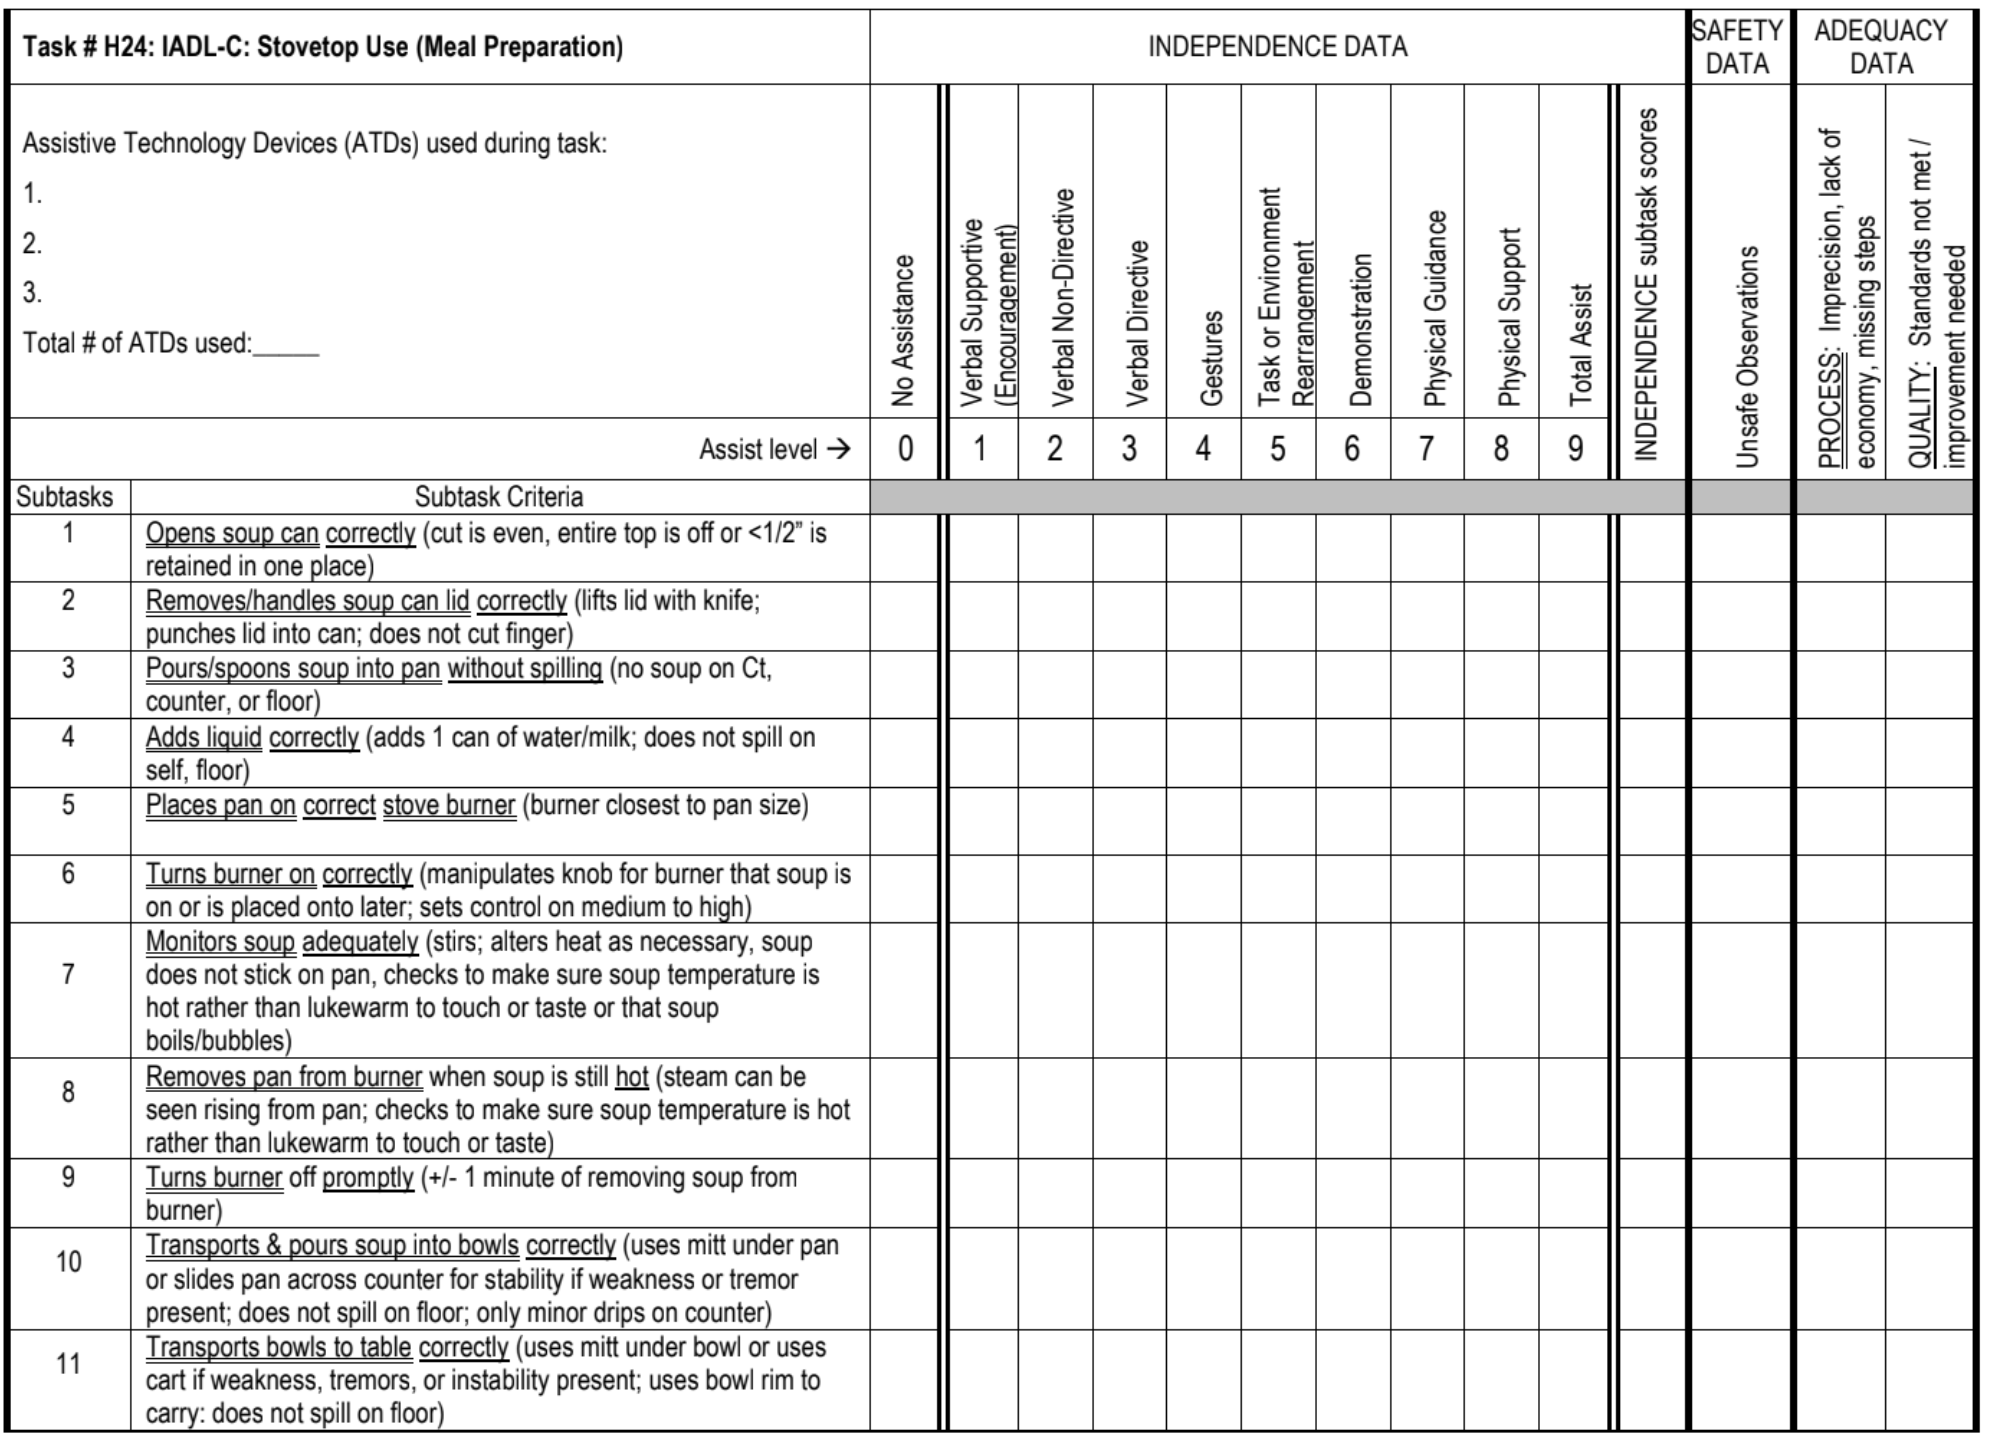
\includegraphics[width=0.8\textwidth]{pass-soup.png}
    \caption{PASS Soup Task \cite{rogers_performance_2014}}
    \label{fig:PASS-soup}
\end{figure}

\begin{figure}[ht]
    \centering
    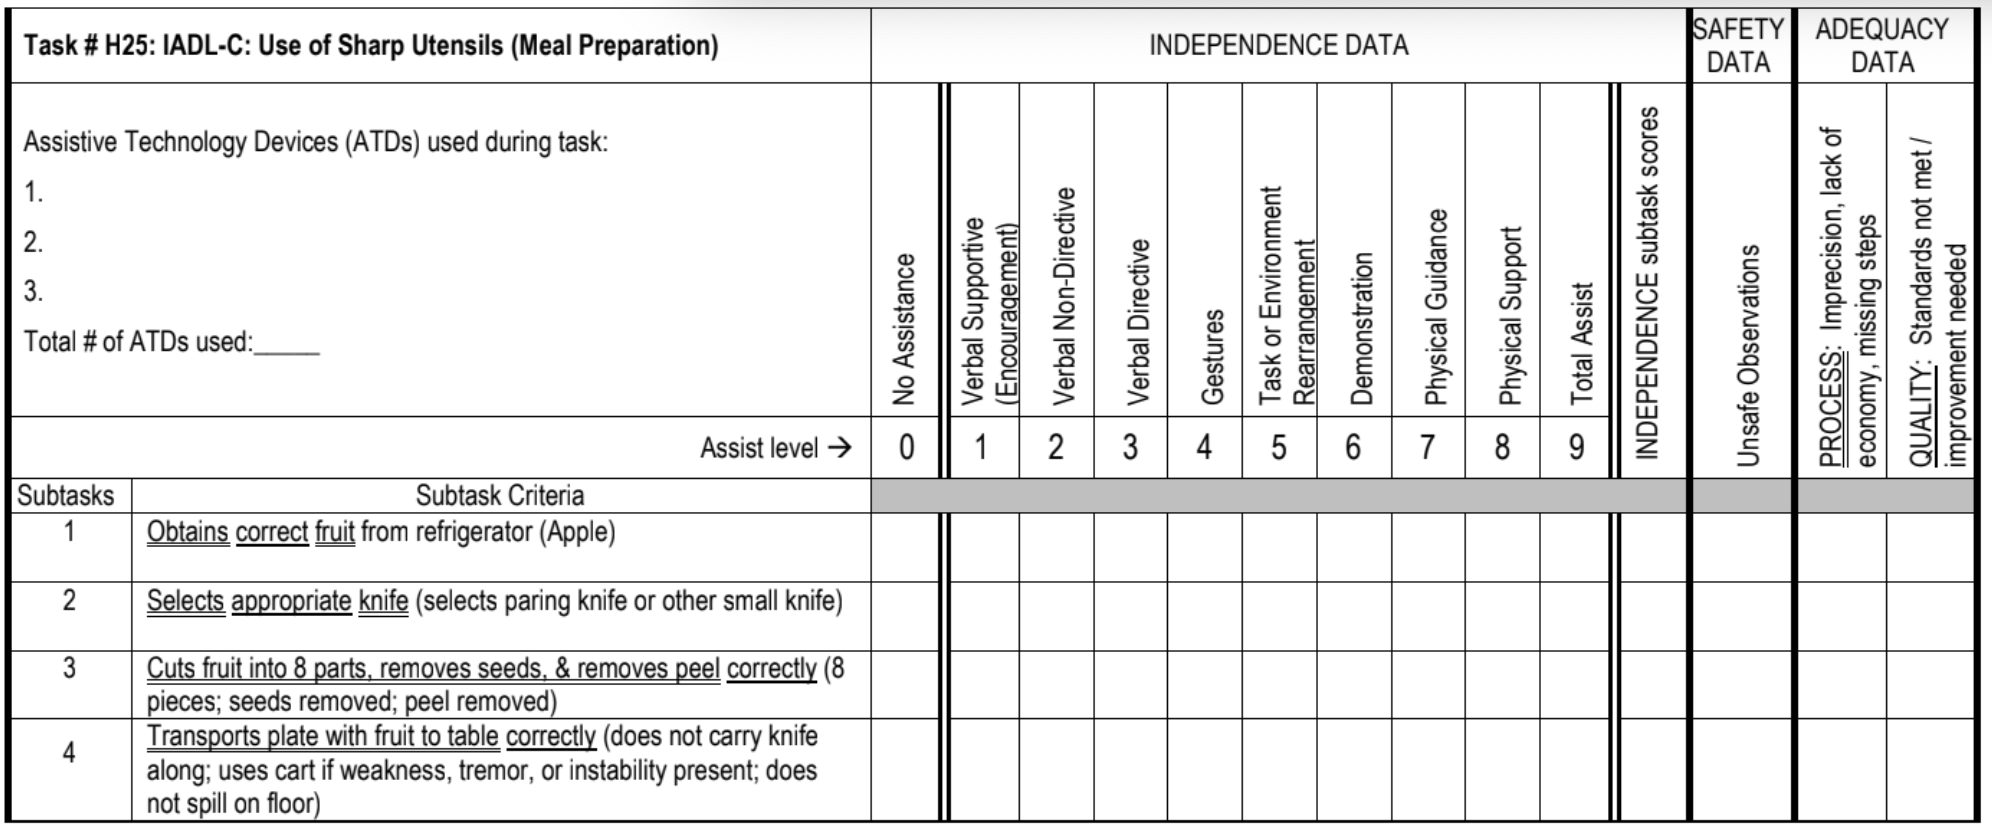
\includegraphics[width=0.8\textwidth]{pass-fruit.png}
    \caption{PASS Fruit Task \cite{rogers_performance_2014}}
    \label{fig:PASS-fruit}
\end{figure}

\begin{figure}[ht]
    \centering
    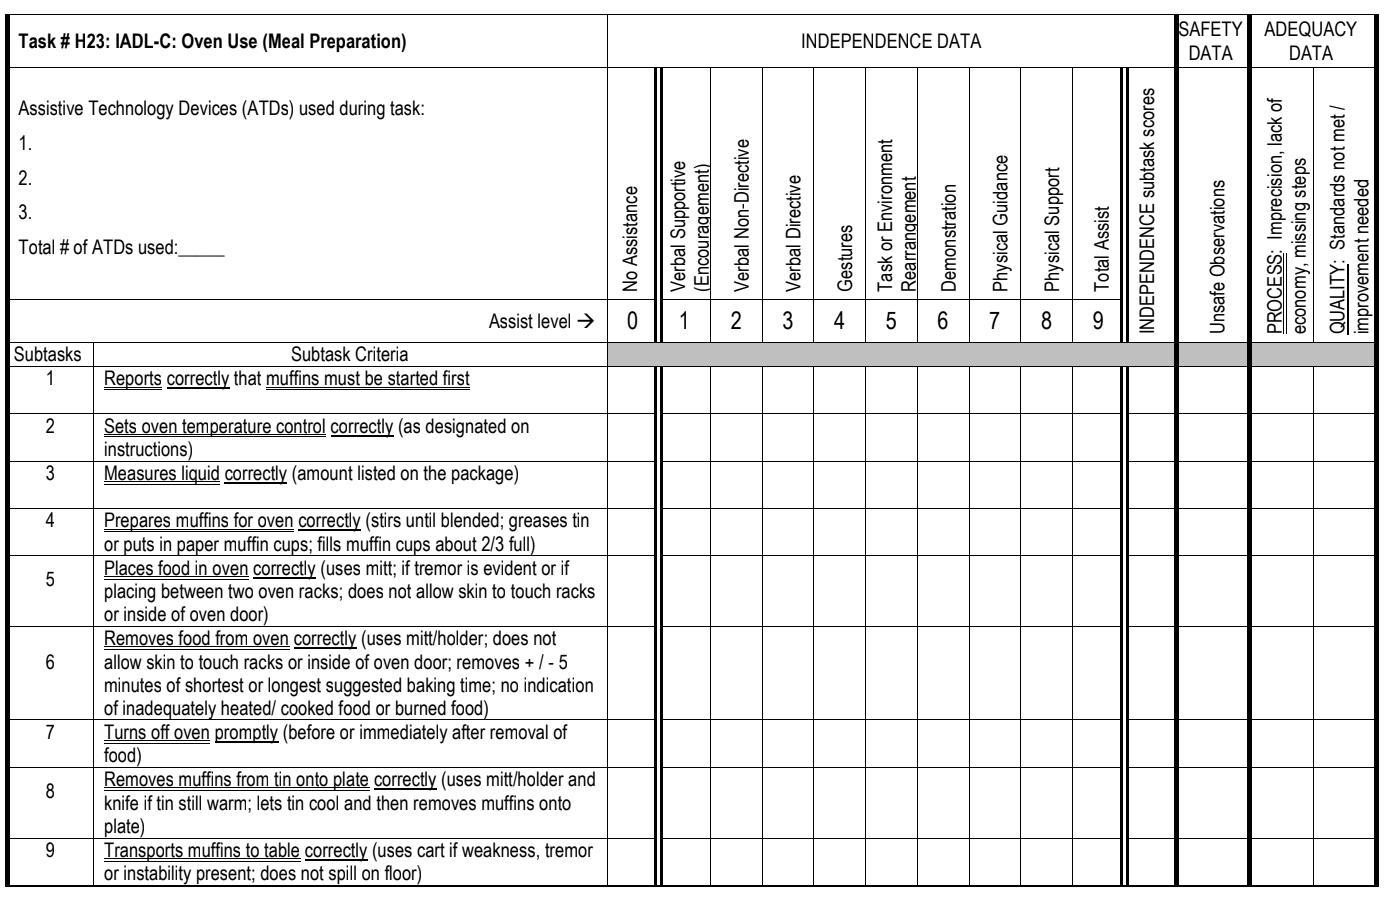
\includegraphics[width=0.8\textwidth]{pass-muffin.png}
    \caption{PASS Muffin Task \cite{rogers_performance_2014}}
    \label{fig:PASS-muffin}
\end{figure}

\clearpage
\section{Fine-grained Task Extraction}
The detail in which tasks can be broken down varies in literature. Human actions may be decomposed all the way into action primitives which is a body part + some motion (eg. right/left hand forward/backward) \cite{huszHumanActivityRecognition2007}. Fine-grained actions can be thought as being one level "coarser" than these action primitives and may combine action primitives to perform a small task (eg. cutting fruit, stir-frying, washing a fruit)  \cite{pan_fine-grained_2020}. A "coarser" level above fine-grained actions are coarse-grained actions and describe the activity that encompasses all of the fine-grained actions (eg. cooking, working). Although action primitives may be useful to consider when breaking down a task, the focus of the thesis is the evaluation of function and ability to perform tasks toward some goal. The detection of coarse-grained actions or activities have been successful in literature previously \cite{cook_learning_2010}, but these coarse-grained actions are too general and do not provide insight into the functional quality of the cooking task. Thus, the focus of the task extraction will be at the "fine-grained" level. 

For each cooking activity in the PASS, an experimental protocol will be developed based on the subtasks outlined in the task document. Although the PASS presents general steps to complete the task, there may sometimes be other actions, or "side-actions" involved in the task. For example, for the Cutting Fruit task in Figure \ref{fig:PASS-fruit}, obtaining the fruit from the refrigerator would require the individual to perform OPEN-FRIDGE, GRAB-FRIDGE, and CLOSE-FRIDGE. The experimental protocol will be more detailed with steps detailing the actions in the PASS as well as any side-actions that occur. Then, from the steps in the experimental protocol, the fine-grained actions can be extracted.

\section{Experimental Protocol}\label{sec:pass-experimental-protocol}
This section will detail the experimental protocol for each of the 3 pass tasks. The steps presented in the original PASS document (Figures \ref{fig:PASS-fruit}-\ref{fig:PASS-muffin}) are used as reference and adapted to the environment where the experiments will take place: the Independent Living Suite. Location of items that were interacted with in the ILS that are not standard in every kitchen are labelled in Figure \ref{fig:ils-item-locs}.

\begin{figure}[ht]
    \centering
    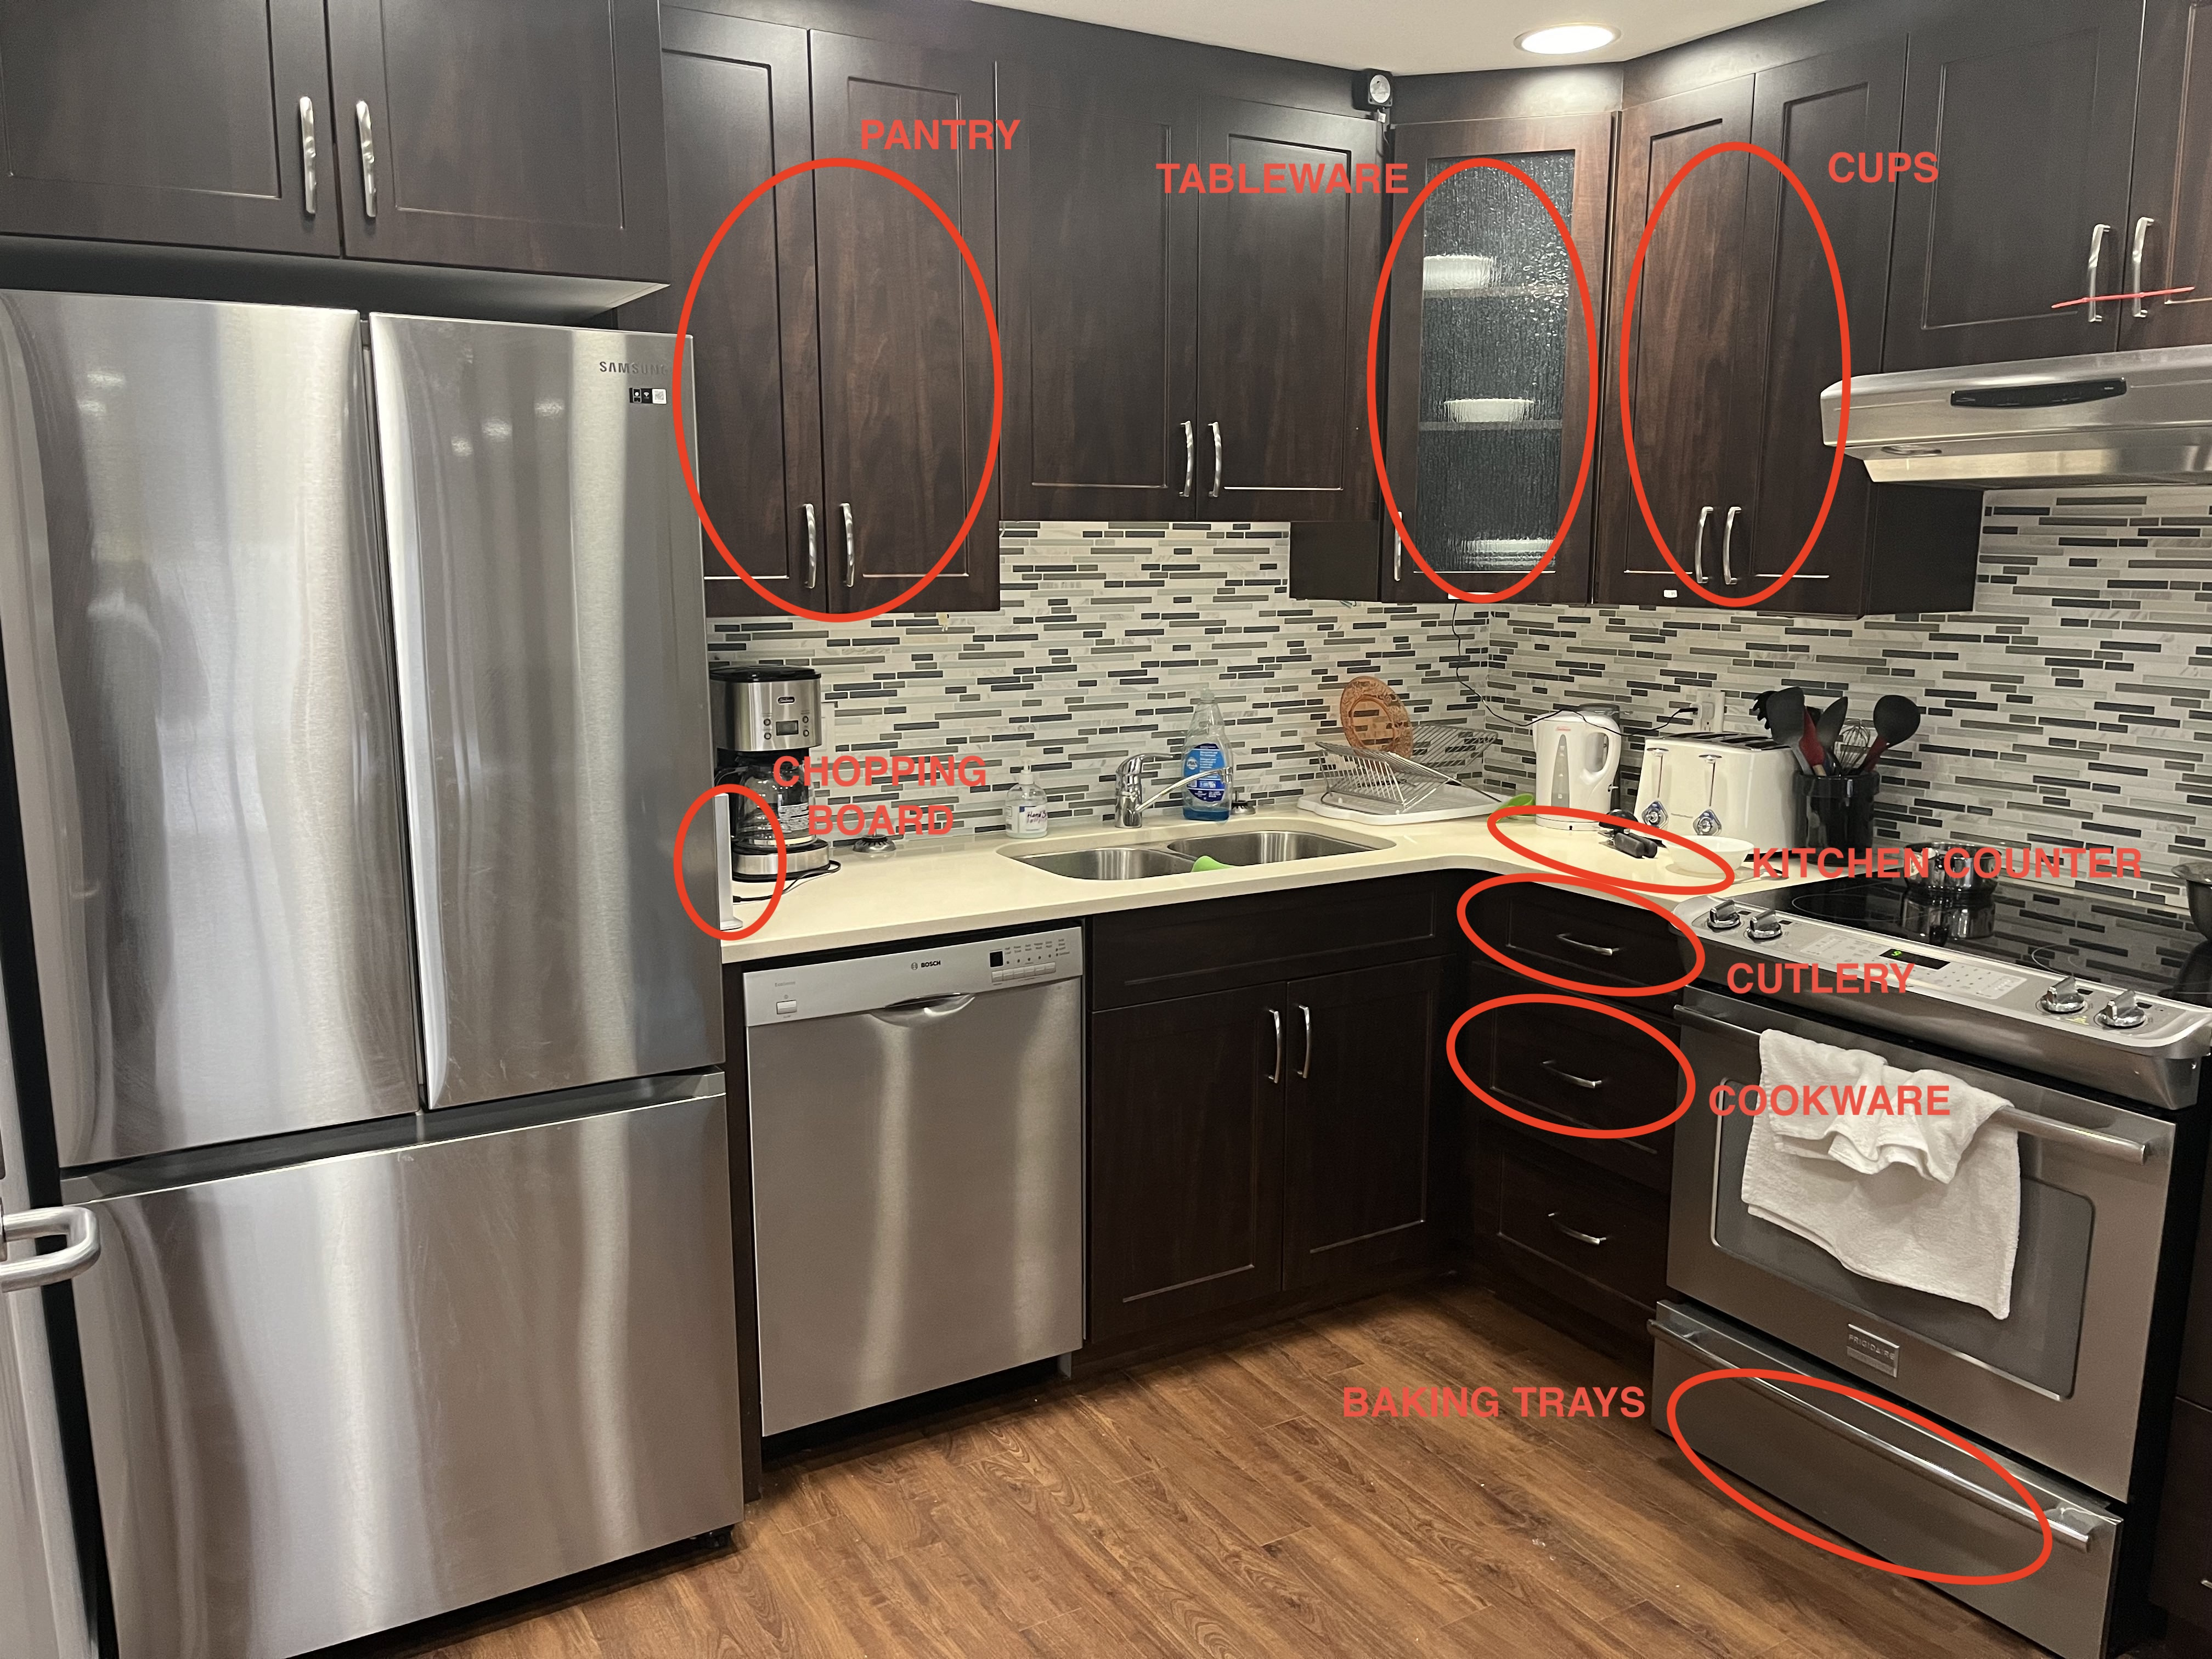
\includegraphics[width=\textwidth]{ils-kitchen-locations.jpg}
    \caption{Independent Living Suite locations.}
    \label{fig:ils-item-locs}
\end{figure}


\subsection{Initial Setup}
The initial setup prior to conducting the experiments involved the following steps:

\subsubsection{Data Recording}
\begin{enumerate}
    \item Referencing the 9H configuration the resulted in the best accuracy and repeatability determined in Chapter \ref{chp:sys-tuning}, the anchors are set up in the locations indicated by Figure \ref{fig:anchorplacement}.
    \item Based on the documentation for the Pozyx \cite{pozyx_configuration_nodate}, the settings for the fastest possible sample rate (16 Hz) without a large effect on the communication range was a bitrate of 850 kbit/s and a preamble length of 128. Both the anchors and the tags were set to communicate at these settings.
    \item Setup a camera with a countdown timer so that segments of the data can be manually labelled at a later time.
    \item Wear the Pozyx tag on the dominant hand.
\end{enumerate}

\subsubsection{Home Conditions}
The home conditions per the PASS Meal Preparation Tasks are listed as the following \cite{rogers_performance_2014}:
\begin{enumerate}
    \item Kitchen area and Electric or gas stove with oven
    \item Sink, “as is”
    \item Usual meal preparation utensils and supplies (e.g., spoons, spatula, bowls, oven mitt/pot holder, etc.)
    \item Apple placed in refrigerator, within easy view when door is opened
    \item Muffin tin for 6 muffins and muffin mix requiring only the addition of water/milk
    \item Can of soup requiring the addition of water/milk
    \item Cookie sheet on kitchen counter nearest stove, with items 5-6 stacked on it
\end{enumerate}

Note that for the following experiments, whenever possible, the dominant hand should be used to perform the actions.

\subsection{Protocol: Cutting Fruit}
Based on Figure \ref{fig:PASS-fruit}, this task involves getting a piece of fruit from the refrigerator, choosing a knife, peeling the fruit, cutting it into 8 pieces, plating and serving it. The detailed steps for the protocol are shown in Table \ref{tab:protocol-cutting-fruit} with the fruit being an apple. Figure \ref{fig:PASS-fruit-setup} shows a part of the setup for the PASS fruit cutting task. Prior to performing the task, the items that the participant interacts with are placed in their original location:

\begin{itemize}
    \item apples - refrigerator
    \item knife - cutlery drawer
    \item plate - tableware cabinet
    \item chopping board - chopping board holder
    \item towel - on oven handle
\end{itemize}

\begin{figure}[ht]
    \centering
    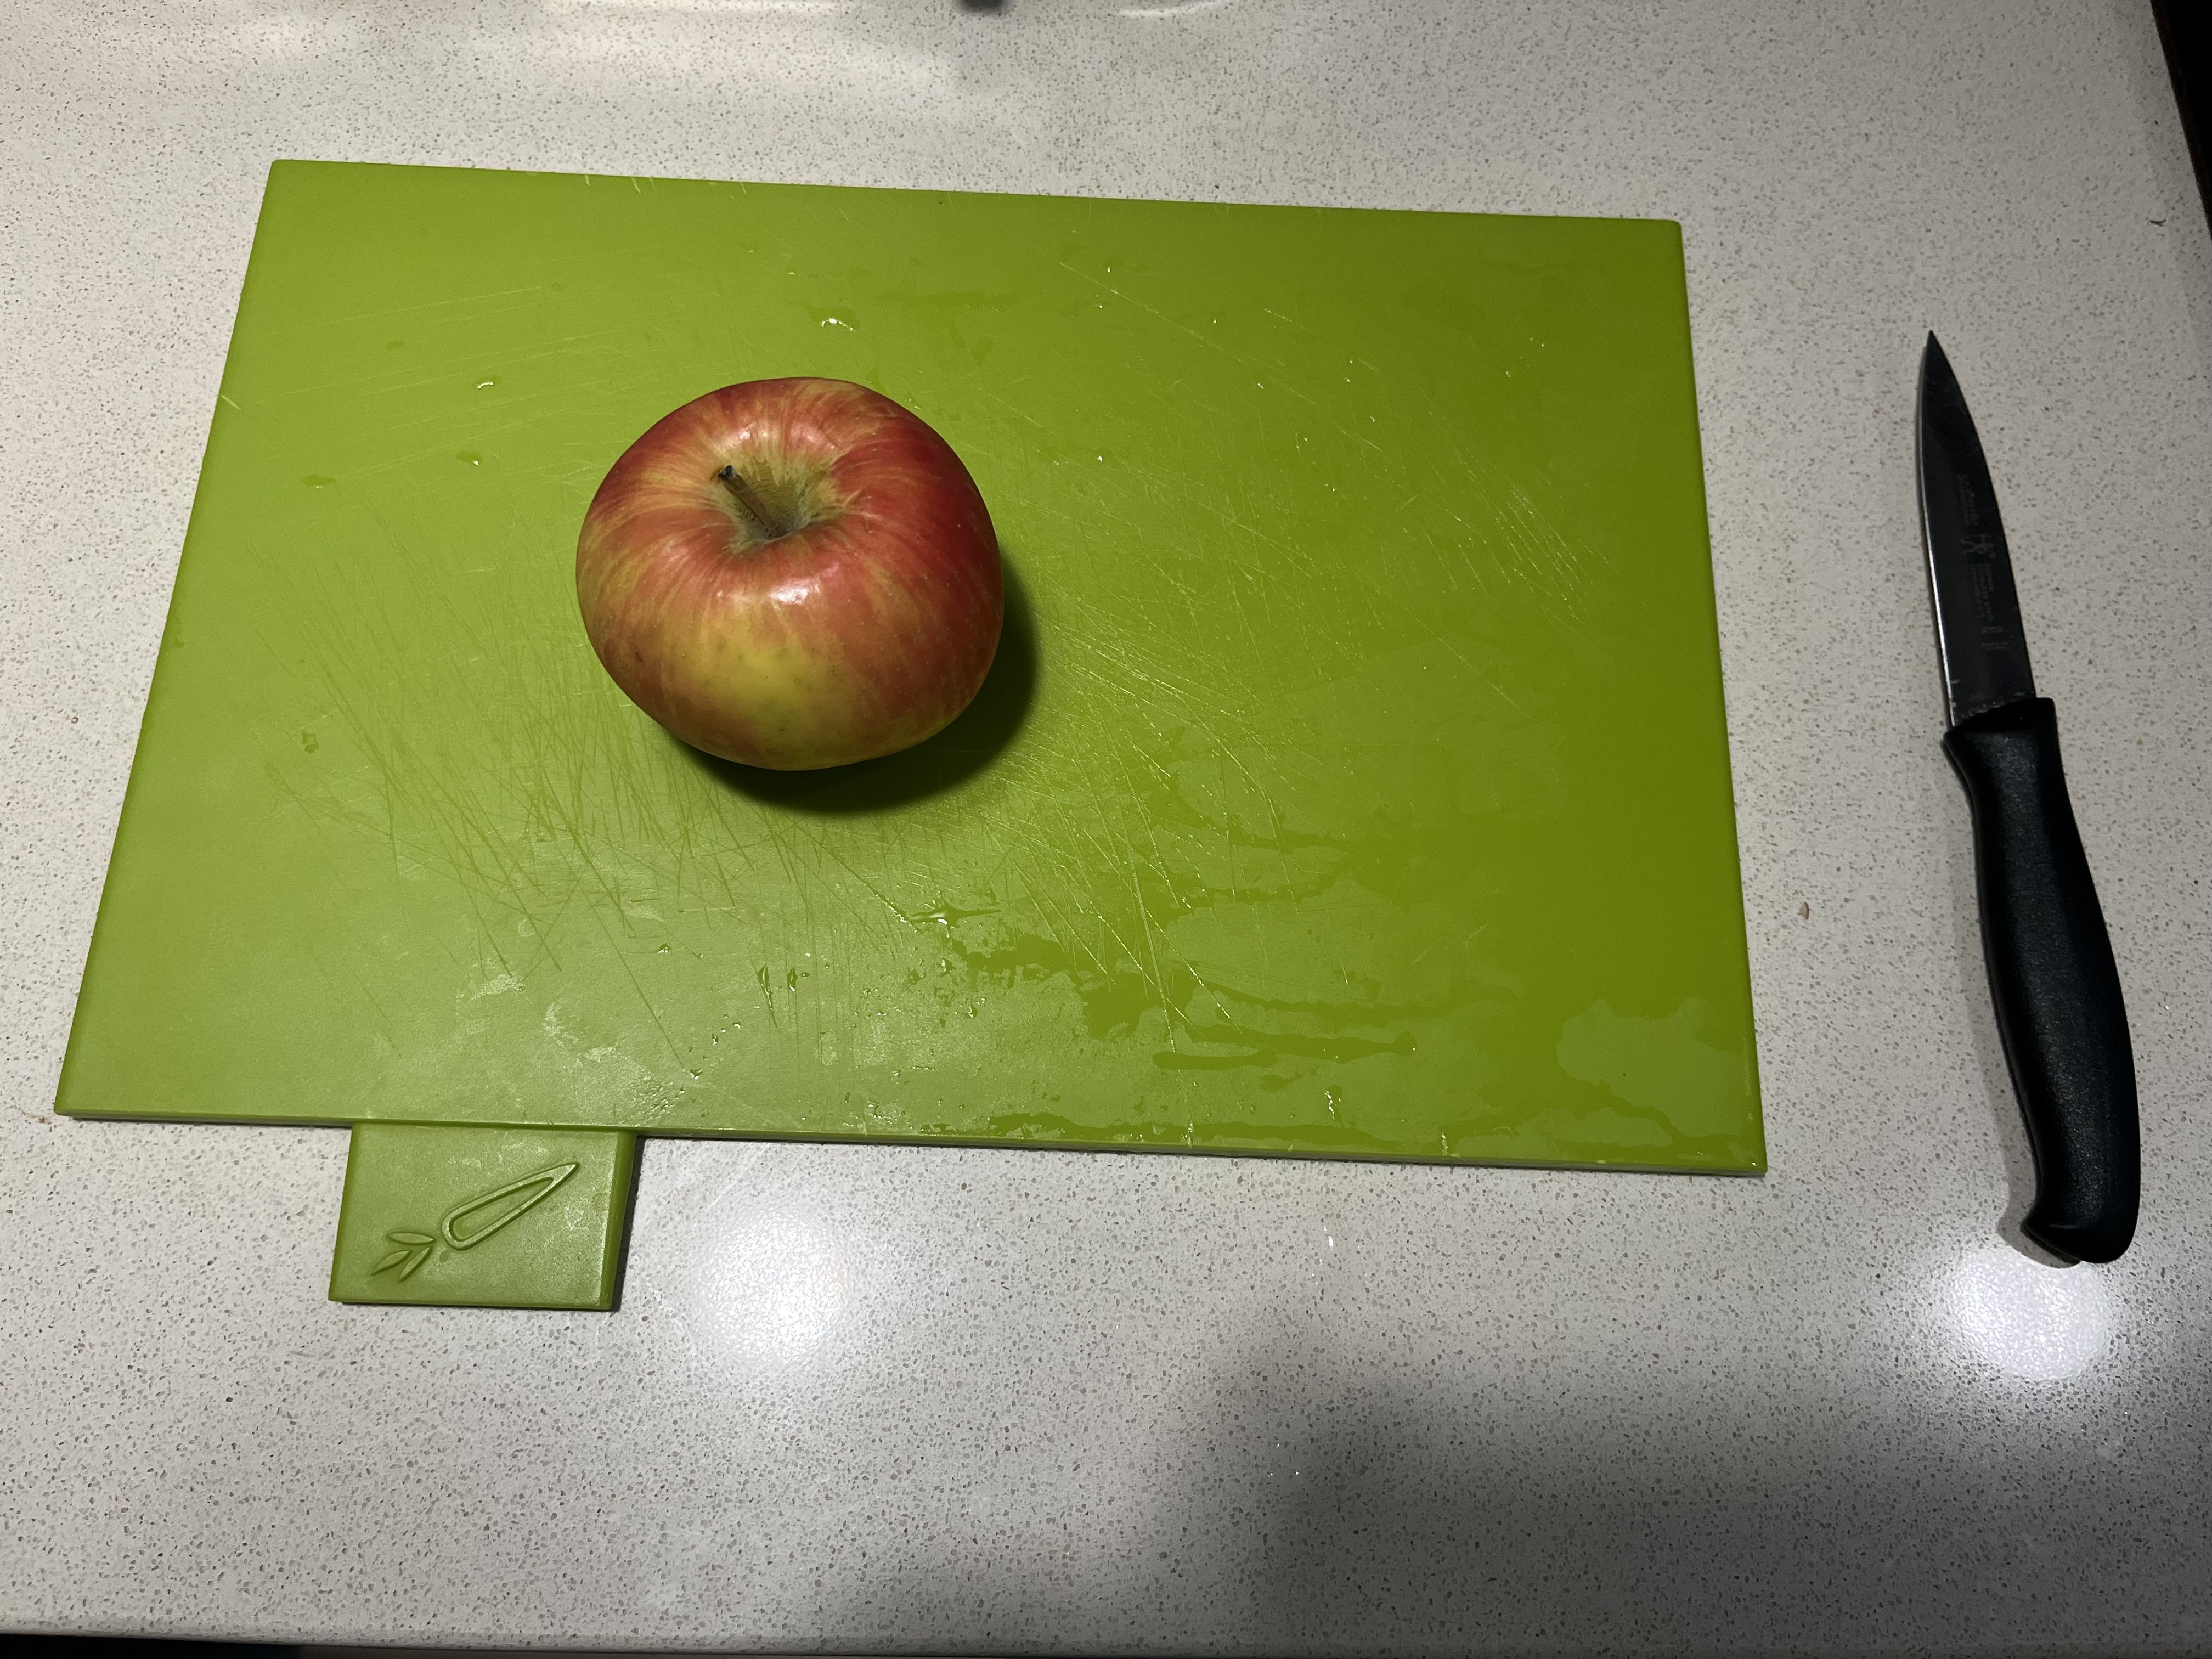
\includegraphics[width=0.8\textwidth]{fruit-setup.jpg}
    \caption{PASS: Fruit Cutting task setup.}
    \label{fig:PASS-fruit-setup}
\end{figure}


{\small
\centering
\renewcommand{\arraystretch}{1.5}
\begin{xltabular}{\textwidth}{>{\hsize=.15\hsize}X X >{\hsize=.4\hsize}X}
\caption{Protocol for the PASS cutting fruit task. Note that Quiet Standing (QS) refers to the position where the participant has their hands on the side of their thighs, being as still as possible.} \label{tab:protocol-cutting-fruit} \\

% First Header
\hline \textbf{Step} & \textbf{Details} & \textbf{Fine-Grained Action} \\ \hline 
\endfirsthead

% Subsequent headers.
\multicolumn{3}{c}{\tablename\ \thetable{} -- continued from previous page} \\
\hline \textbf{Step} & \textbf{Details} & \textbf{Fine-Grained Action} \\ \hline 
\endhead

% Footers
\hline \multicolumn{3}{r}{\textit{Continued on next page}} \\ \hline
\endfoot

% Last Footer
\hline
\endlastfoot

% The Table
    1 & Start the video with the countdown and just as the countdown finishes start data collection script & \\ 
    2 & Move to the position in front of the refrigerator and stand in a Quiet Standing (QS) position for 2-3 seconds. Quickly raise and lower the hand with the sensor (for sensor and video time synchronization) and return to QS & \\ 
    3 & Stay in QS for 5 seconds & QS \\
    4 & Walk to the sink & \\
    5 & Open the faucet and wash hands for 10 seconds, close the faucet & WASH \\
    6 & Walk to the position in front of the oven (where the drying towel is) &  \\
    7 & Dry hands & DRY \\
    8 & Walk to the position in front of the refrigerator & \\
    9 & Open the refrigerator with the dominant hand & OPEN-FRIDGE \\
    10 & Reach into the fridge and grab an apple with the dominant hand & GRAB-FRIDGE \\
    11 & Close the fridge with the dominant hand & CLOSE-FRIDGE \\
    12 & Place the apple on the kitchen counter & \\
    13 & Walk to where the cutting board is & \\
    14 & Grab the cutting board with the dominant hand & GRAB-BOARD \\
    15 & Walk to the kitchen counter & \\
    16 & Place the cutting board on the kitchen counter (beside the apple) & \\
    17 & Move to the position in front of the drawer containing the knife & \\
    18 & Open the drawer with the knife with the dominant hand & OPEN-CUTLERY \\
    19 & Grab the parring knife with the dominant hand & GRAB-CUTLERY \\
    20 & Close the drawer with the dominant hand & CLOSE-CUTLERY \\
    21 & Place the knife on the counter & \\
    22 & Grab the apple and move to the position in front of the sink & \\
    23 & Wash the apple & WASH \\
    24 & Move back to the position in front of the counter &  \\
    25 & Peel the apple using the parring knife & PEEL \\
    26 & Cut the apple into 8ths using the chopping board & CUT \\
    27 & Move to the position in front of the tableware cabinet & \\
    28 & Open the tableware cabinet door with the dominant hand & OPEN-TABLEWARE \\
    29 & Grab a plate and place it on the kitchen counter & GRAB-TABLEWARE \\
    30 & Close the tableware cabinet with the dominant hand & CLOSE-TABLEWARE \\
    31 & Move to the position in front of the kitchen counter & \\
    32 & Transfer the apple slices from the cutting board to the plate with the dominant hand & PLATING \\
    33 & Grab the plate with the apples and bring it to the dining table & SERVE \\
    34 & Return to the position in front of the refrigerator and stand in QS for 5 seconds & QS \\
    35 & End data collection and end the recording & \\
    \hline
\end{xltabular}
}

\clearpage
\subsection{Protocol: Making Soup}

Based on Figure \ref{fig:PASS-soup}, this task involves preparing soup from a soup can. The individual must locate the soup can in the pantry, open it and prepare it according to the instructions. The preparation of a soup can typically involves measuring and adding a liquid such as milk or water to the contents in the soup can and warming it up on the stove top. The detailed steps are documented in Table \ref{tab:protocol-making-soup}. Similar to the cutting fruit task, the items (shown in Figure \ref{fig:PASS-soup-items}) that the participant interacts with must be placed back in their original position:

\begin{itemize}
    \item soup can - pantry
    \item towel - on oven handle
    \item can opener - cutlery cabinet
    \item spoon - cutlery drawer
    \item pot - cookware drawer
    \item bowl - tableware cabinet
\end{itemize}

\begin{figure}[ht]
    \centering
    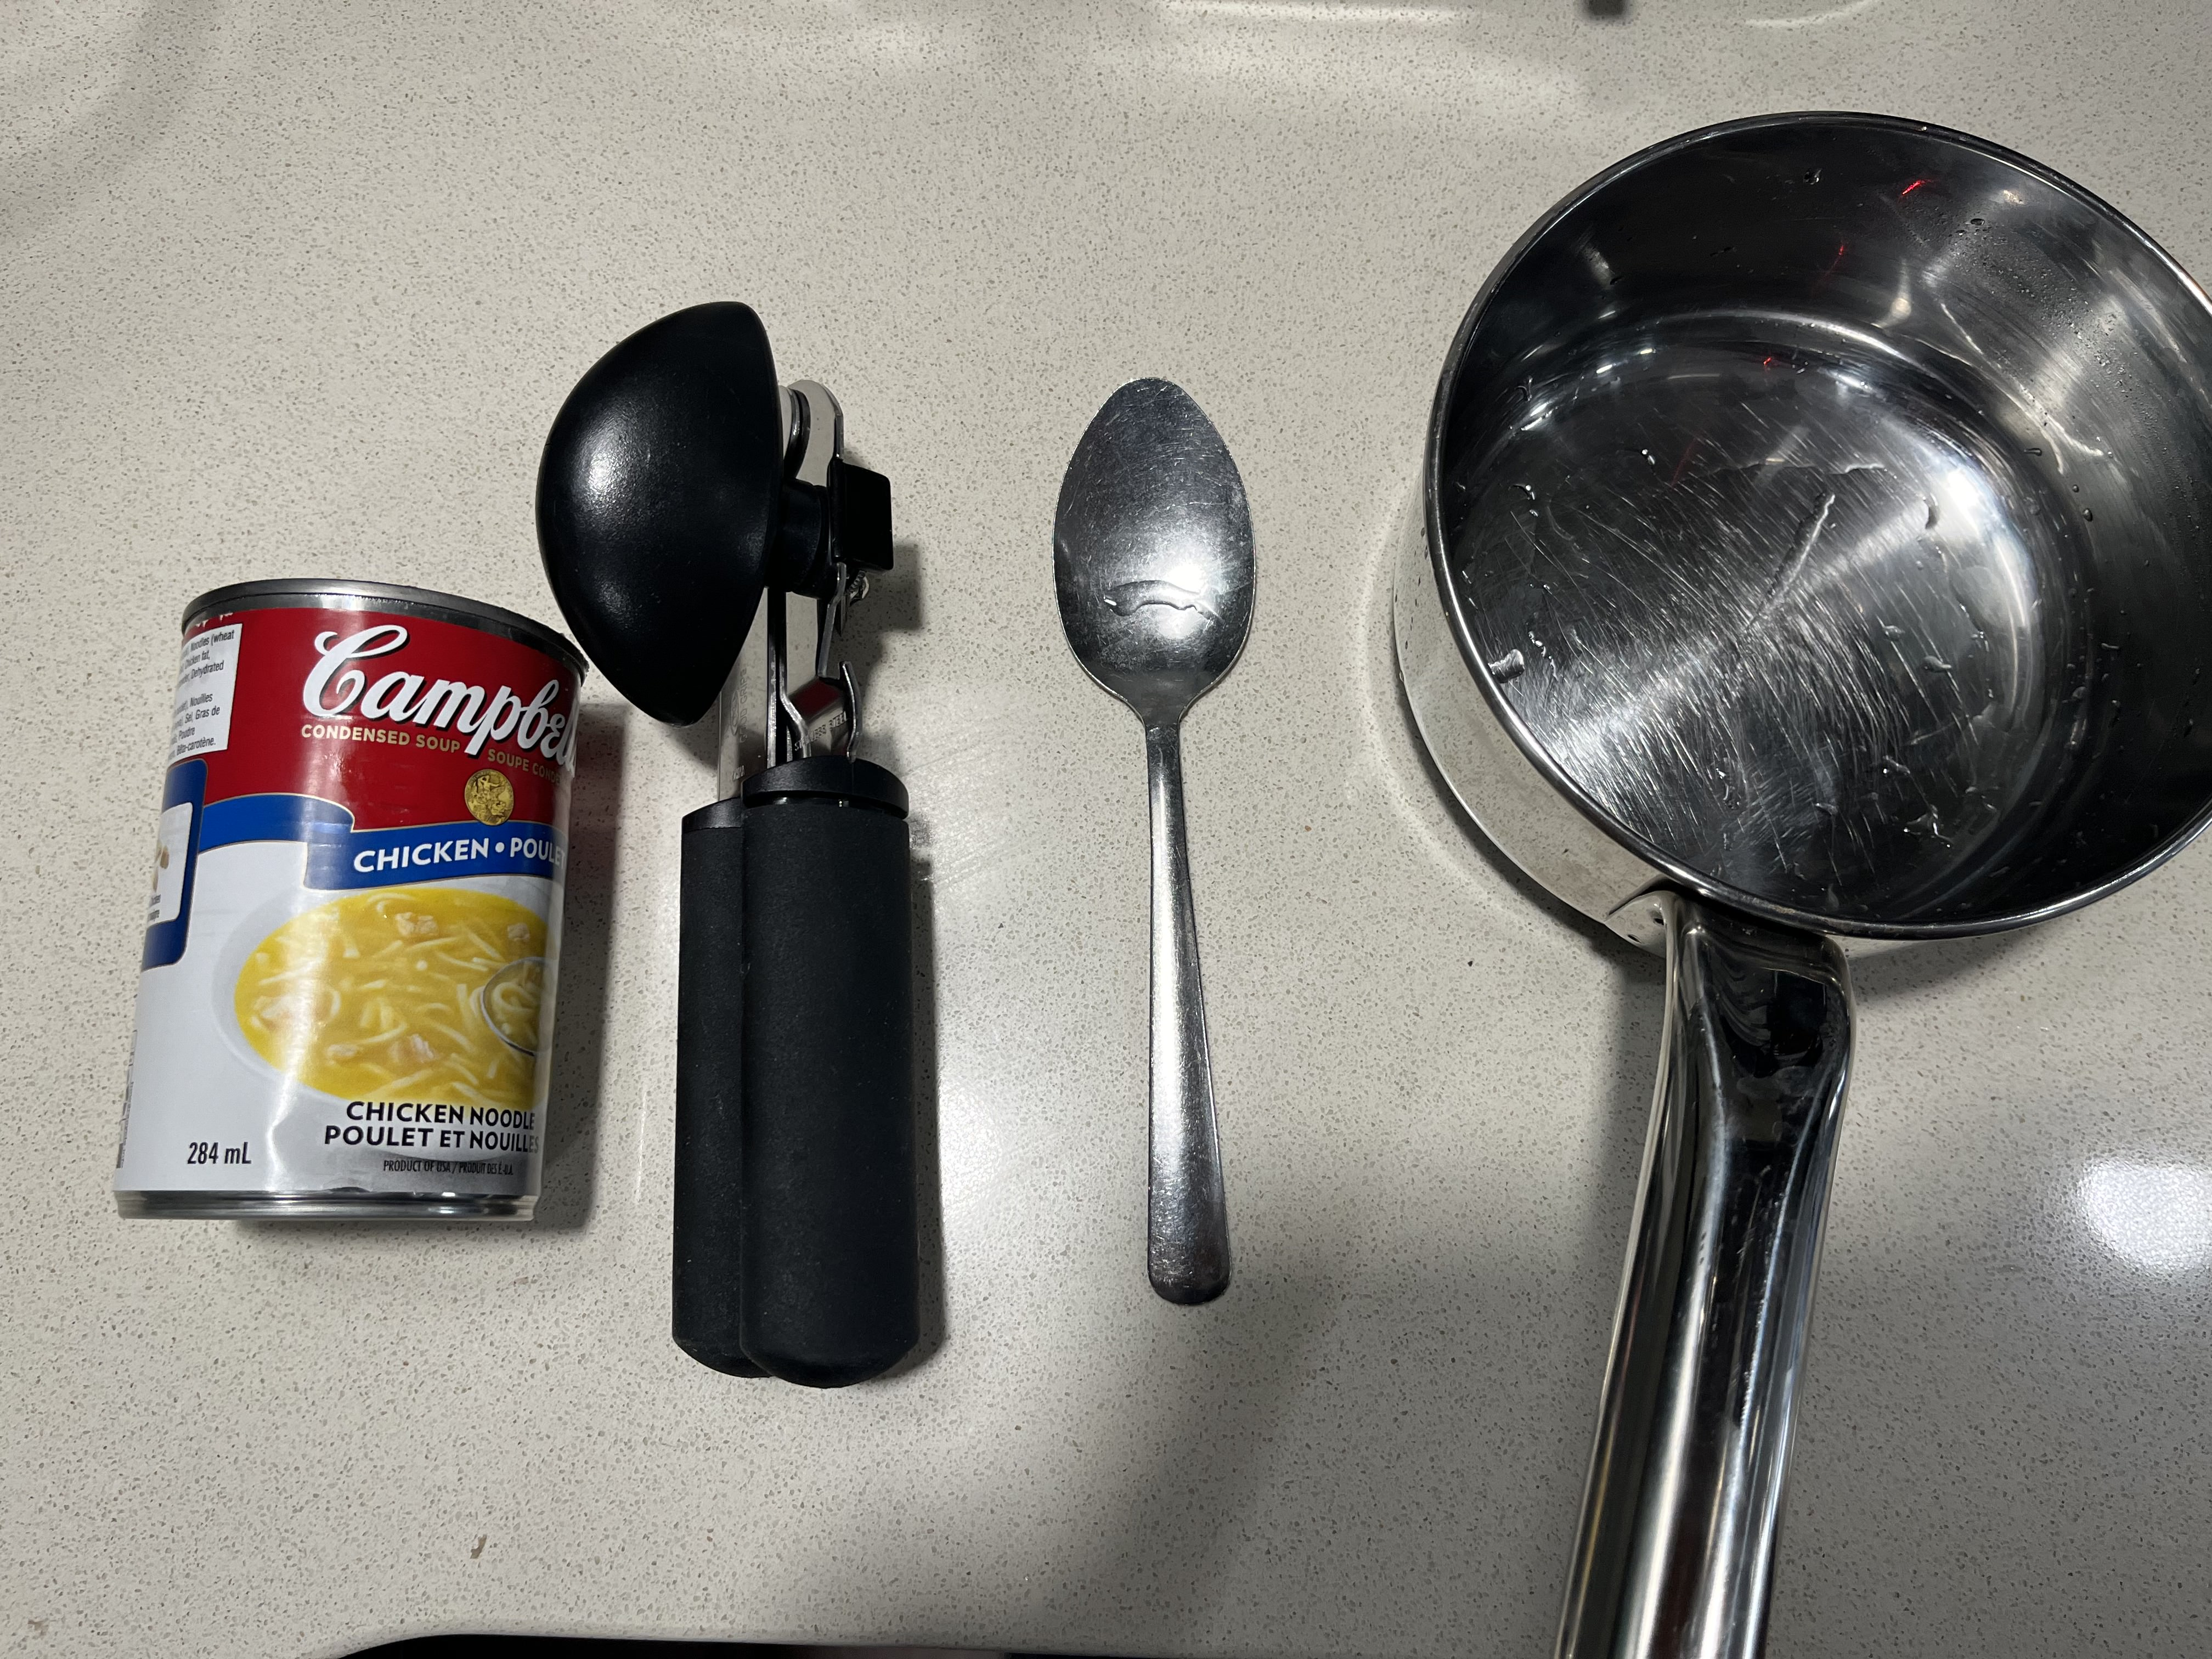
\includegraphics[width=0.8\textwidth]{makesoup-items.jpg}
    \caption{Items used in the PASS make soup task. From the left: the can of soup, can opener, spoon and pot.}
    \label{fig:PASS-soup-items}
\end{figure}

{\small
\centering
\renewcommand{\arraystretch}{1.5}
\clearpage
\begin{xltabular}{\textwidth}{>{\hsize=.15\hsize}X X >{\hsize=.4\hsize}X}
\caption{Protocol for the PASS making soup task. Note that Quiet Standing (QS) refers to the position where the participant has their hands on the side of their thighs, being as still as possible.} \label{tab:protocol-making-soup} \\

% First Header
\hline \textbf{Step} & \textbf{Details} & \textbf{Fine-Grained Action} \\ \hline 
\endfirsthead

% Subsequent headers.
\multicolumn{3}{c}{\tablename\ \thetable{} -- continued from previous page} \\
\hline \textbf{Step} & \textbf{Details} & \textbf{Fine-Grained Action} \\ \hline 
\endhead

% Footers
\hline \multicolumn{3}{r}{\textit{Continued on next page}} \\ \hline
\endfoot

% Last Footer
\hline
\endlastfoot

% The Table
    1  & Start the video with the countdown and just as the countdown finishes start data collection script & \\ 
    2  & Move to the position in front of the refrigerator and stand in a Quiet Standing (QS) position for 2-3 seconds. Quickly raise and lower the hand with the sensor (for sensor and video time synchronization) and return to QS & \\ 
    3  & Stay in QS for 5 seconds & QS \\
    4  & Walk to the sink & \\
    5  & Open the faucet and wash hands for 10 seconds, close the faucet & WASH \\
    6  & Walk to the position in front of the oven (where the drying towel is) &  \\
    7  & Dry hands & DRY \\
    8  & Move to the position in front of the pantry cabinet & \\
    9  & Open the pantry cabinet with the dominant hand & OPEN-PANTRY \\
    10 & Grab the soup can inside the pantry cabinet with the dominant hand & GRAB-PANTRY \\
    11 & Close the pantry cabinet with the dominant hand & CLOSE-PANTRY \\
    12 & Bring the soup can to the kitchen counter and set it on the counter & \\
    13 & Move to the position in front of the cutlery drawer & \\
    14 & Open the cutlery drawer with the dominant hand & OPEN-CUTLERY \\
    15 & Grab the spoon and the can opener in the cutlery drawer and place them on the counter & GRAB-CUTLERY \\
    16 & Close the cutlery drawer with the dominant hand & CLOSE-CUTLERY \\
    17 & Move to the position in front of the cookware drawer & \\
    18 & Open the cookware drawer with the dominant hand & OPEN-COOKWARE \\
    19 & Grab the pot from the cookware drawer and place it on the counter & GRAB-COOKWARE \\
    20 & Close the cookware drawer with the dominant hand & CLOSE-COOKWARE \\
    21 & Move to the position in front of the kitchen counter & \\
    22 & Using the can opener, open the can of soup with the dominant hand & OPEN-CAN \\
    23 & Pour the contents into the pot with the dominant hand & POUR \\
    24 & While holding the empty can, move to the position in front of the sink &  \\
    25 & Fill the soup can to the top with tap water with the dominant hand & FILL-WATER \\
    26 & Move back to the position in front of the kitchen counter & \\
    27 & Pour the water into the pot containing the concentrated soup with the dominant hand & POUR \\
    28 & Grab the pot and move to the position in front of the stove with the dominant hand & \\
    29 & Place the pot on one of the burners & \\
    30 & Turn the burner on with the dominant hand & BURNER-ON \\
    31 & Move back about a meter and stand in QS for about 10 seconds to mimic waiting for the soup to boil & QS \\
    32 & Grab the spoon on the counter and use it to stir the soup for about 10 seconds with the dominant hand & STIR \\
    33 & Turn the burner off & BURNER-OFF \\
    34 & Move to the position in front of the tableware cabinet & \\
    35 & Open the tableware cabinet door with the dominant hand & OPEN-TABLEWARE \\
    36 & Grab a bowl and place it on the kitchen counter & GRAB-TABLEWARE \\
    37 & Close the tableware cabinet with the dominant hand & CLOSE-TABLEWARE \\
    38 & Move to the position in front of the stove and grab the pot & \\
    39 & Move to the position in front of the cabinet with the pot & \\
    40 & Pour the soup in the pot into the bowl (being careful not to spill any) with the dominant hand & POUR \\
    41 & Grab the bowl of soup and bring it to the dining table & SERVE \\
    42 & Return to the position in front of the refrigerator and stand in QS for 5 seconds & QS \\
    43 & End data collection and end the recording & \\
    \hline
\end{xltabular}
}

\clearpage
\subsection{Protocol: Making Muffins}
From Figure \ref{fig:PASS-muffin}, this PASS task evaluates the older adult's ability to use the oven through baking muffins. The muffin batter is made using pre-made muffin mix to minimize the number of steps required in gathering the ingredients per the PASS task instructions. The participant is required to make the muffin batter, pour the batter into the muffin tin for 6 muffins and place the muffin tin into the oven. To simulate a speed up in the baking process, a pre-baked 6 pack of muffin has been placed in the oven before hand and used as the finished product for plating and serving. Items used in this experiment are shown in Figure \ref{fig:PASS-muffin-items} Detailed steps are found in Table \ref{tab:protocol-making-muffins}. Similar to the making soup task, the items (shown in Figure \ref{fig:PASS-muffin-items}) that the participant interacts with must be placed back in their original position:

\begin{itemize}
    \item muffin mix - pantry
    \item towel - on oven handle
    \item measuring cup - cutlery drawer
    \item tongs - cutlery drawer
    \item spoon - cutlery drawer
    \item mixing bowl - cookware drawer
    \item muffin tin - baking trays drawer
    \item water measuring cup - cups cabinet
    \item oven mitts - cookware drawer
    \item 6-pack pre-baked muffins - inside the oven, to one side
\end{itemize}

\begin{figure}[ht]
    \centering
    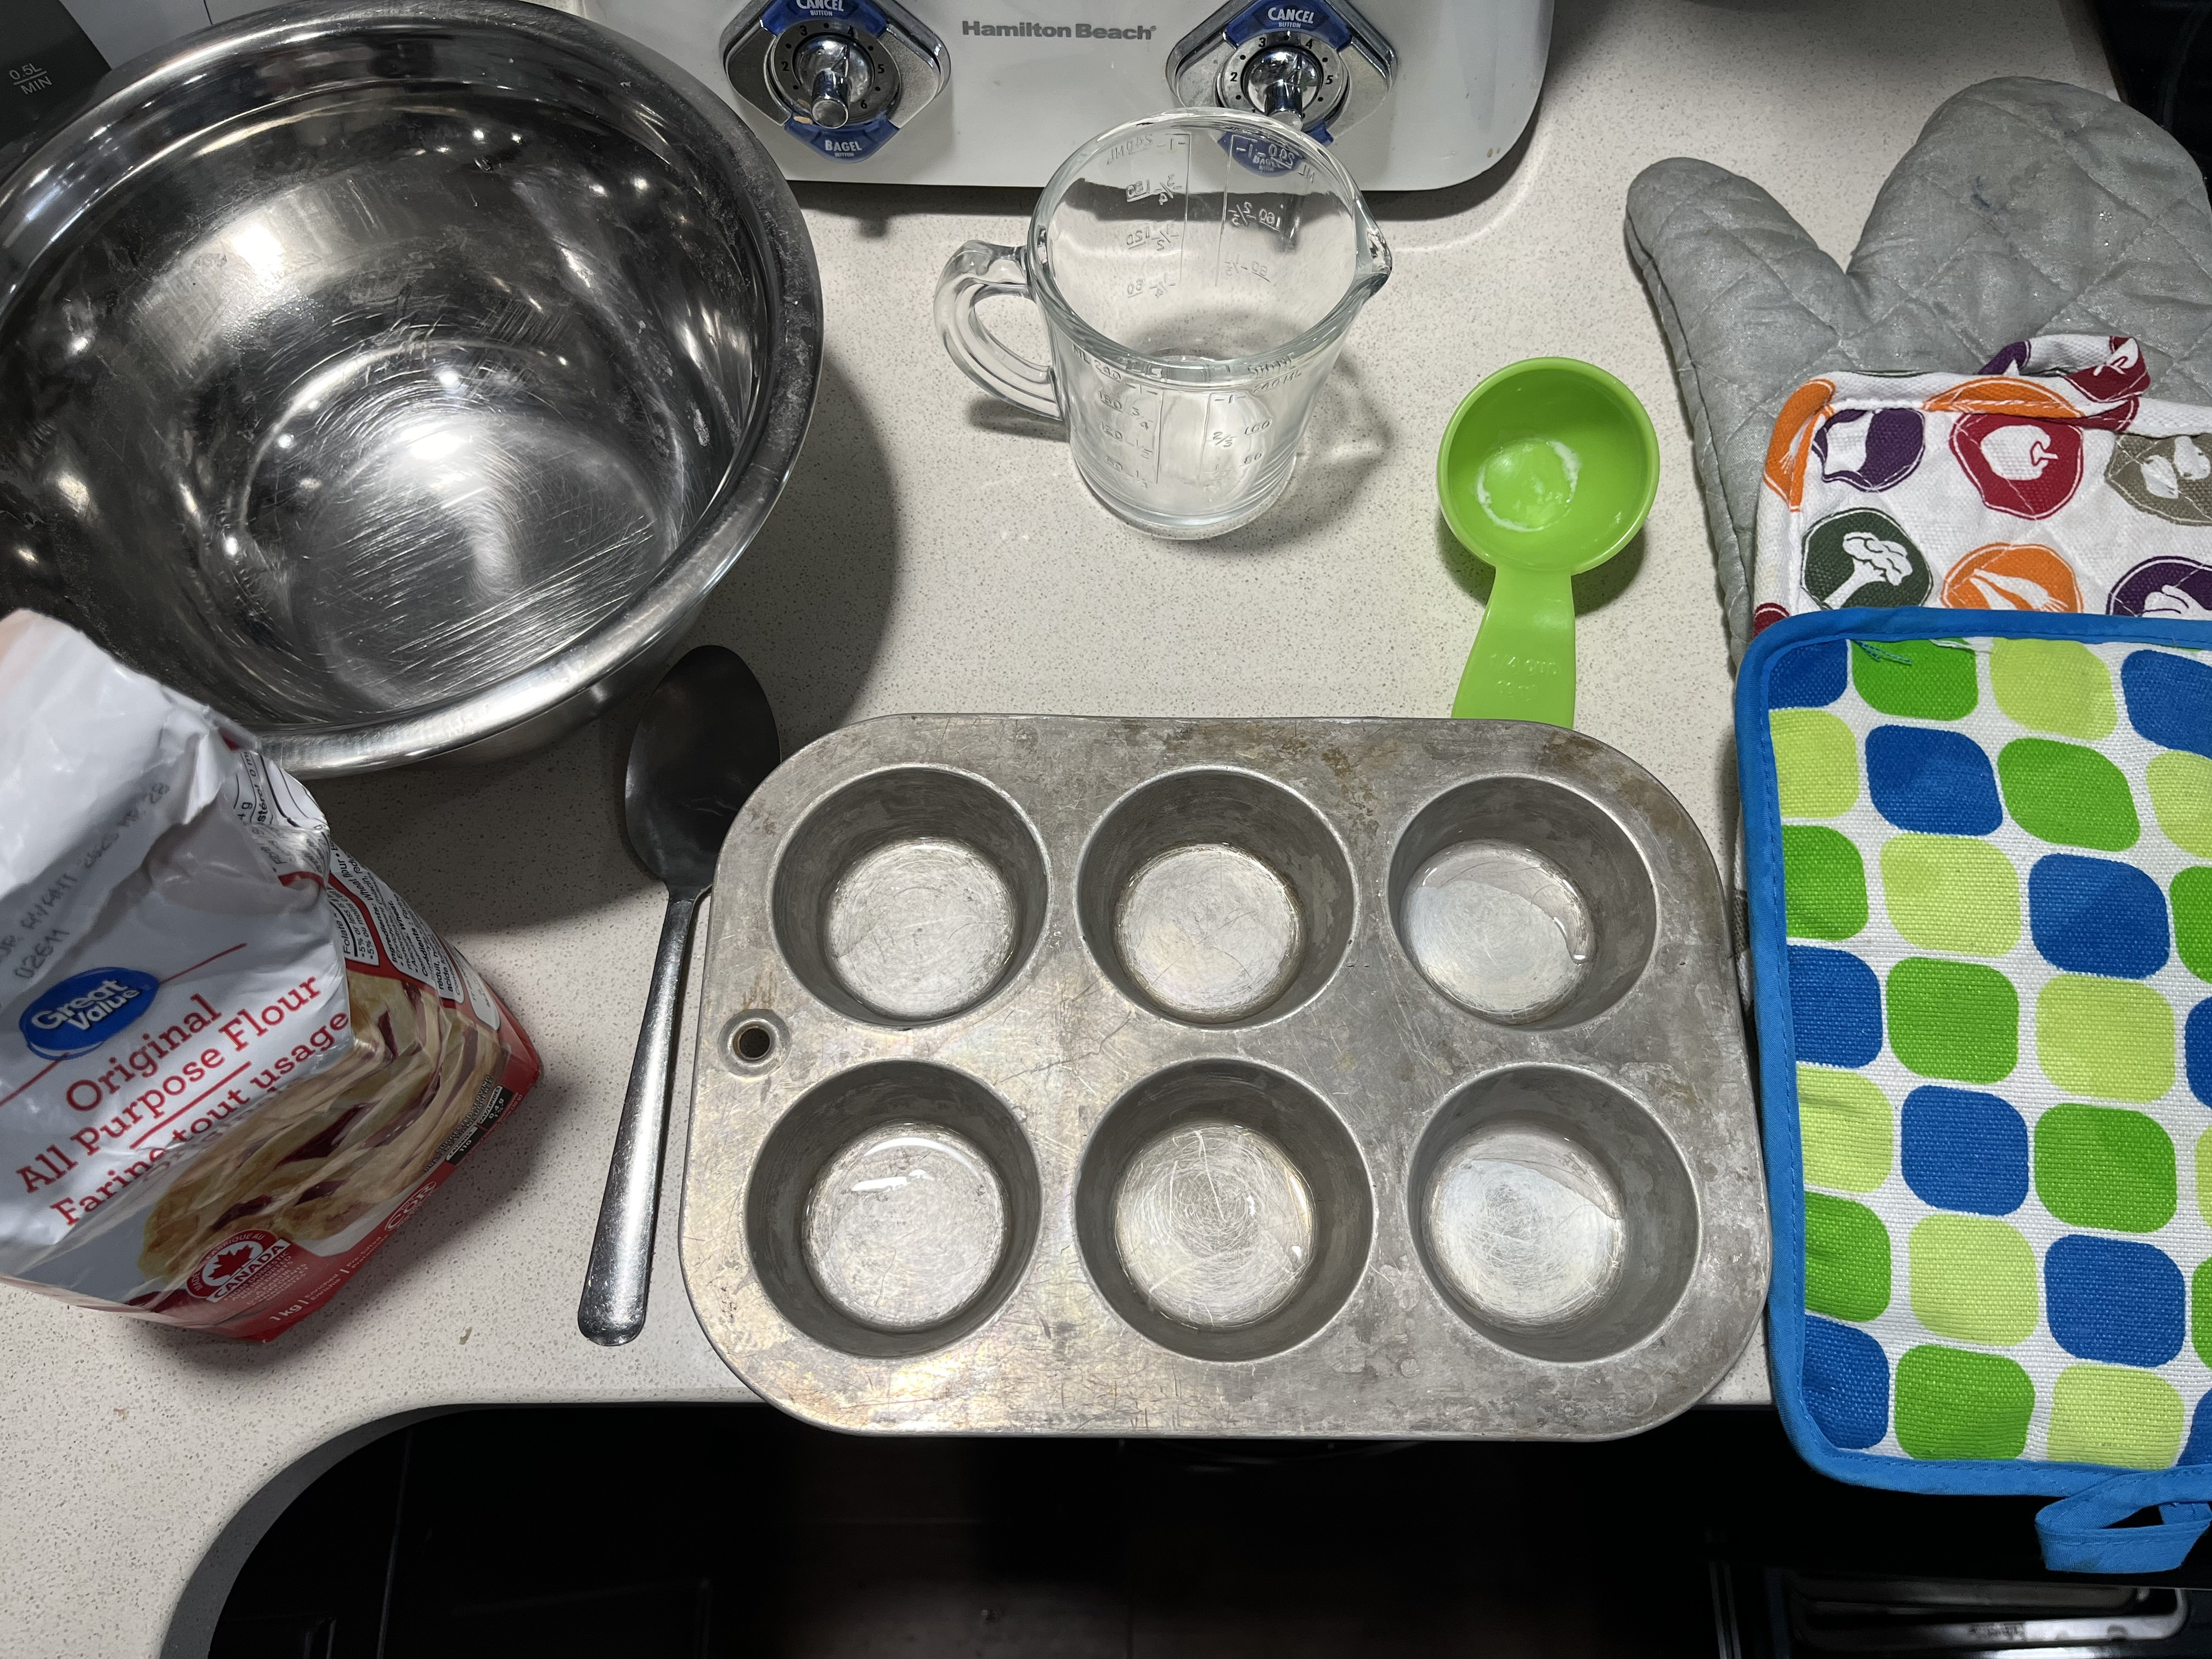
\includegraphics[width=0.8\textwidth]{baking-muffin-items.jpg}
    \caption{Items used in the Baking Muffin task. From the left: the muffin mix, the mixing bowl, the spoon, the muffin tin, the water measuring cup, the (green) measuring cup, and assorted oven mitts. The 6 pack of muffins and tongs are not shown in the image, but can be found at any local super market and kitchen supply store respectively.}
    \label{fig:PASS-muffin-items}
\end{figure}

{\small
\centering
\renewcommand{\arraystretch}{1.5}
\clearpage
\begin{xltabular}{\textwidth}{>{\hsize=.15\hsize}X X >{\hsize=.4\hsize}X}
\caption{Protocol for the PASS making muffins task. Note that Quiet Standing (QS) refers to the position where the participant has their hands on the side of their thighs, being as still as possible.} \label{tab:protocol-making-muffins} \\

% First Header
\hline \textbf{Step} & \textbf{Details} & \textbf{Fine-Grained Action} \\ \hline 
\endfirsthead

% Subsequent headers.
\multicolumn{3}{c}{\tablename\ \thetable{} -- continued from previous page} \\
\hline \textbf{Step} & \textbf{Details} & \textbf{Fine-Grained Action} \\ \hline 
\endhead

% Footers
\hline \multicolumn{3}{r}{\textit{Continued on next page}} \\ \hline
\endfoot

% Last Footer
\hline
\endlastfoot

% The Table
    1  & Start the video with the countdown and just as the countdown finishes start data collection script & \\ 
    2  & Move to the position in front of the refrigerator and stand in a Quiet Standing (QS) position for 2-3 seconds. Quickly raise and lower the hand with the sensor (for sensor and video time synchronization) and return to QS & \\ 
    3  & Stay in QS for 5 seconds & QS \\
    4  & Walk to the sink & \\
    5  & Open the faucet and wash hands for 10 seconds, close the faucet & WASH \\
    6  & Walk to the position in front of the oven (where the drying towel is) &  \\
    7  & Dry hands & DRY \\
    8  & Move to the position in front of the pantry cabinet & \\
    9  & Open the pantry cabinet with the dominant hand & OPEN-PANTRY \\
    10 & Grab the muffin mix in the pantry with the dominant hand & GRAB-PANTRY \\
    11 & Close the pantry cabinet with the dominant hand & CLOSE-PANTRY \\
    12 & Bring the muffin mix kitchen counter and set it on the counter & \\
    13 & Move to the position in front of the cutlery drawer & \\
    14 & Open the cutlery drawer with the dominant hand & OPEN-CUTLERY \\
    15 & Grab the spoon and the measuring cup in the cutlery drawer and place them on the counter & GRAB-CUTLERY \\
    16 & Close the cutlery drawer with the dominant hand & CLOSE-CUTLERY \\
    17 & Move to the position in front of the cups cabinet & \\
    18 & Open the cup cabinet with the dominant hand & OPEN-CUPS \\
    19 & Grab the water measuring cup with the dominant hand & GRAB-CUPS \\
    20 & Close the cup cabinet with the dominant hand & GRAB-CUPS \\
    21 & Move to the position in front of the cookware drawer & \\
    22 & Open the cookware drawer with the dominant hand & OPEN-COOKWARE \\
    23 & Grab the mixing bowl from the cookware drawer and place it on the counter & GRAB-COOKWARE \\
    24 & Close the cookware drawer with the dominant hand & CLOSE-COOKWARE \\
    25 & Move to the position in front of the kitchen counter & \\
    26 & Open the muffin mix and grab the measuring cup with the dominant hand & \\
    27 & Scoop the required amount of muffin mix into the mixing bowl & SCOOP \\
    28 & Put down the measuring cup and grab the water measuring cup with the dominant hand & \\
    29 & While holding the empty water measuring cup, move to the position in front of the sink &  \\
    30 & Fill the water measuring cup can to the required level (per muffin mix directions) with tap water & FILL-WATER \\
    31 & Move back to the position in front of the kitchen counter & \\
    32 & Pour the water in the water measuring cup into the mixing bowl containing the muffin mix & POUR \\
    33 & Put down the water measuring cup and grab the spoon & \\
    34 & Mix the water and muffin mix together in the mixing bowl using a stirring motion & STIR \\
    35 & Put the spoon down and move to the position in front of the drawer for the baking trays &  \\
    36 & Open the baking tray drawer with the dominant hand & OPEN-BAKING-TRAYS \\
    37 & Grab the muffin tin from the drawer with the dominant hand & GRAB-BAKING-TRAYS \\
    38 & Close the baking tray drawer with the dominant hand & CLOSE-BAKING-TRAYS \\
    39 & Bring the tray to the kitchen counter and set it close to the mixing bowl & \\
    40 & Grab the measuring cup with the dominant hand & \\
    41 & Scoop the muffin batter in the mixing bowl into the muffin tin & SCOOP \\
    42 & Move in front of the oven & \\
    43 & Simulate turning on the oven (do not actually turn it on) with the dominant hand & OVEN-POWER \\
    44 & Step backwards around 1 meter away from the oven and stand in QS for about 10 seconds to mimic waiting for the oven to preheat & QS \\
    45 & Once the oven has "pre-heated" move back to the position in front of the oven & \\
    46 & Open the oven using the dominant hand & OPEN-OVEN \\
    47 & Grab the muffin tin with the muffin batter and place it into one of the oven racks & GRAB-OVEN \\
    48 & Close the oven with the dominant hand & CLOSE-OVEN \\
    49 & Step backwards around 1 meter away from the oven and stand in QS for about 10 seconds to mimic waiting for the muffins to bake & QS \\
    50 & Move back in front of the oven & \\
    51 & Simulate turning off the oven with the dominant hand & OVEN-POWER \\
    52 & Move in front of the cookware drawer & \\
    53 & Open the cookware drawer with the dominant hand & OPEN-COOKWARE \\
    54 & Grab some oven mitts that are in the cookware drawer & GRAB-COOKWARE \\
    55 & Close the cookware drawer with the dominant hand & CLOSE-COOKWARE \\
    56 & Put on the oven mitts & \\
    57 & Move to the position in front of the oven & \\
    58 & Open the oven with the dominant hand & OPEN-OVEN \\
    59 & Reach in and grab the pre-made 6-pack of muffins with the dominant hand and place the muffins on the stovetop (because in a real baking scenario it should be hot) & GRAB-OVEN \\
    60 & Close the oven with the dominant hand & CLOSE-OVEN \\
    61 & Take the oven mitts off and move to the position in front of the cookware drawer & \\
    62 & Open the cookware drawer with the dominant hand & OPEN-COOKWARE \\
    63 & Place the oven mitts into the cookware drawer & GRAB-COOKWARE \\
    64 & Close the cookware drawer with the dominant hand & CLOSE-COOKWARE \\
    65 & Move to the position in front of the cutler drawer & \\
    66 & Open the cutlery drawer with the dominant hand & OPEN-CUTLERY \\
    67 & Grab the tongs from the cutlery drawer with the dominant hand & GRAB-CUTLERY \\
    68 & Close the cutlery drawer with the dominant hand & CLOSE-CUTLERY \\
    69 & Move to the position in front of the tableware cabinet & \\
    70 & Open the tableware cabinet door with the dominant hand & OPEN-TABLEWARE \\
    71 & Grab a plate and place it on the kitchen counter & GRAB-TABLEWARE \\
    72 & Close the tableware cabinet with the dominant hand & CLOSE-TABLEWARE \\
    73 & Move to the position in front of the kitchen counter & \\
    74 & Use the tongs to transfer 3 muffins from the "muffin tin" to the plate & PLATING \\
    75 & Put the tongs down & \\                        
    76 & Grab the plate with the muffins on it and bring it to the dining table & SERVE \\
    77 & Return to the position in front of the refrigerator and stand in QS for 5 seconds & QS \\
    78 & End data collection and end the recording & \\ 
    \hline
\end{xltabular}
}

\clearpage
\section{Disability Simulation}
To both further the amount of data collected as well as increase the variation in the data, 3 disability simulations will be used while following the experimental protocol described in Section \ref{sec:pass-experimental-protocol}. Figure \ref{fig:disability-simulation} shows the items used to simulate the disabilities and the disability simulations are as follows:

\begin{enumerate}
    \item Vision Impairment: Covering one eye
    \item Mild Physical Impairment: Wearing Knitted Gloves
    \item Severe Physical Impairment: Wearing Electrical Gloves
\end{enumerate}

\begin{figure}[ht]
    \centering
    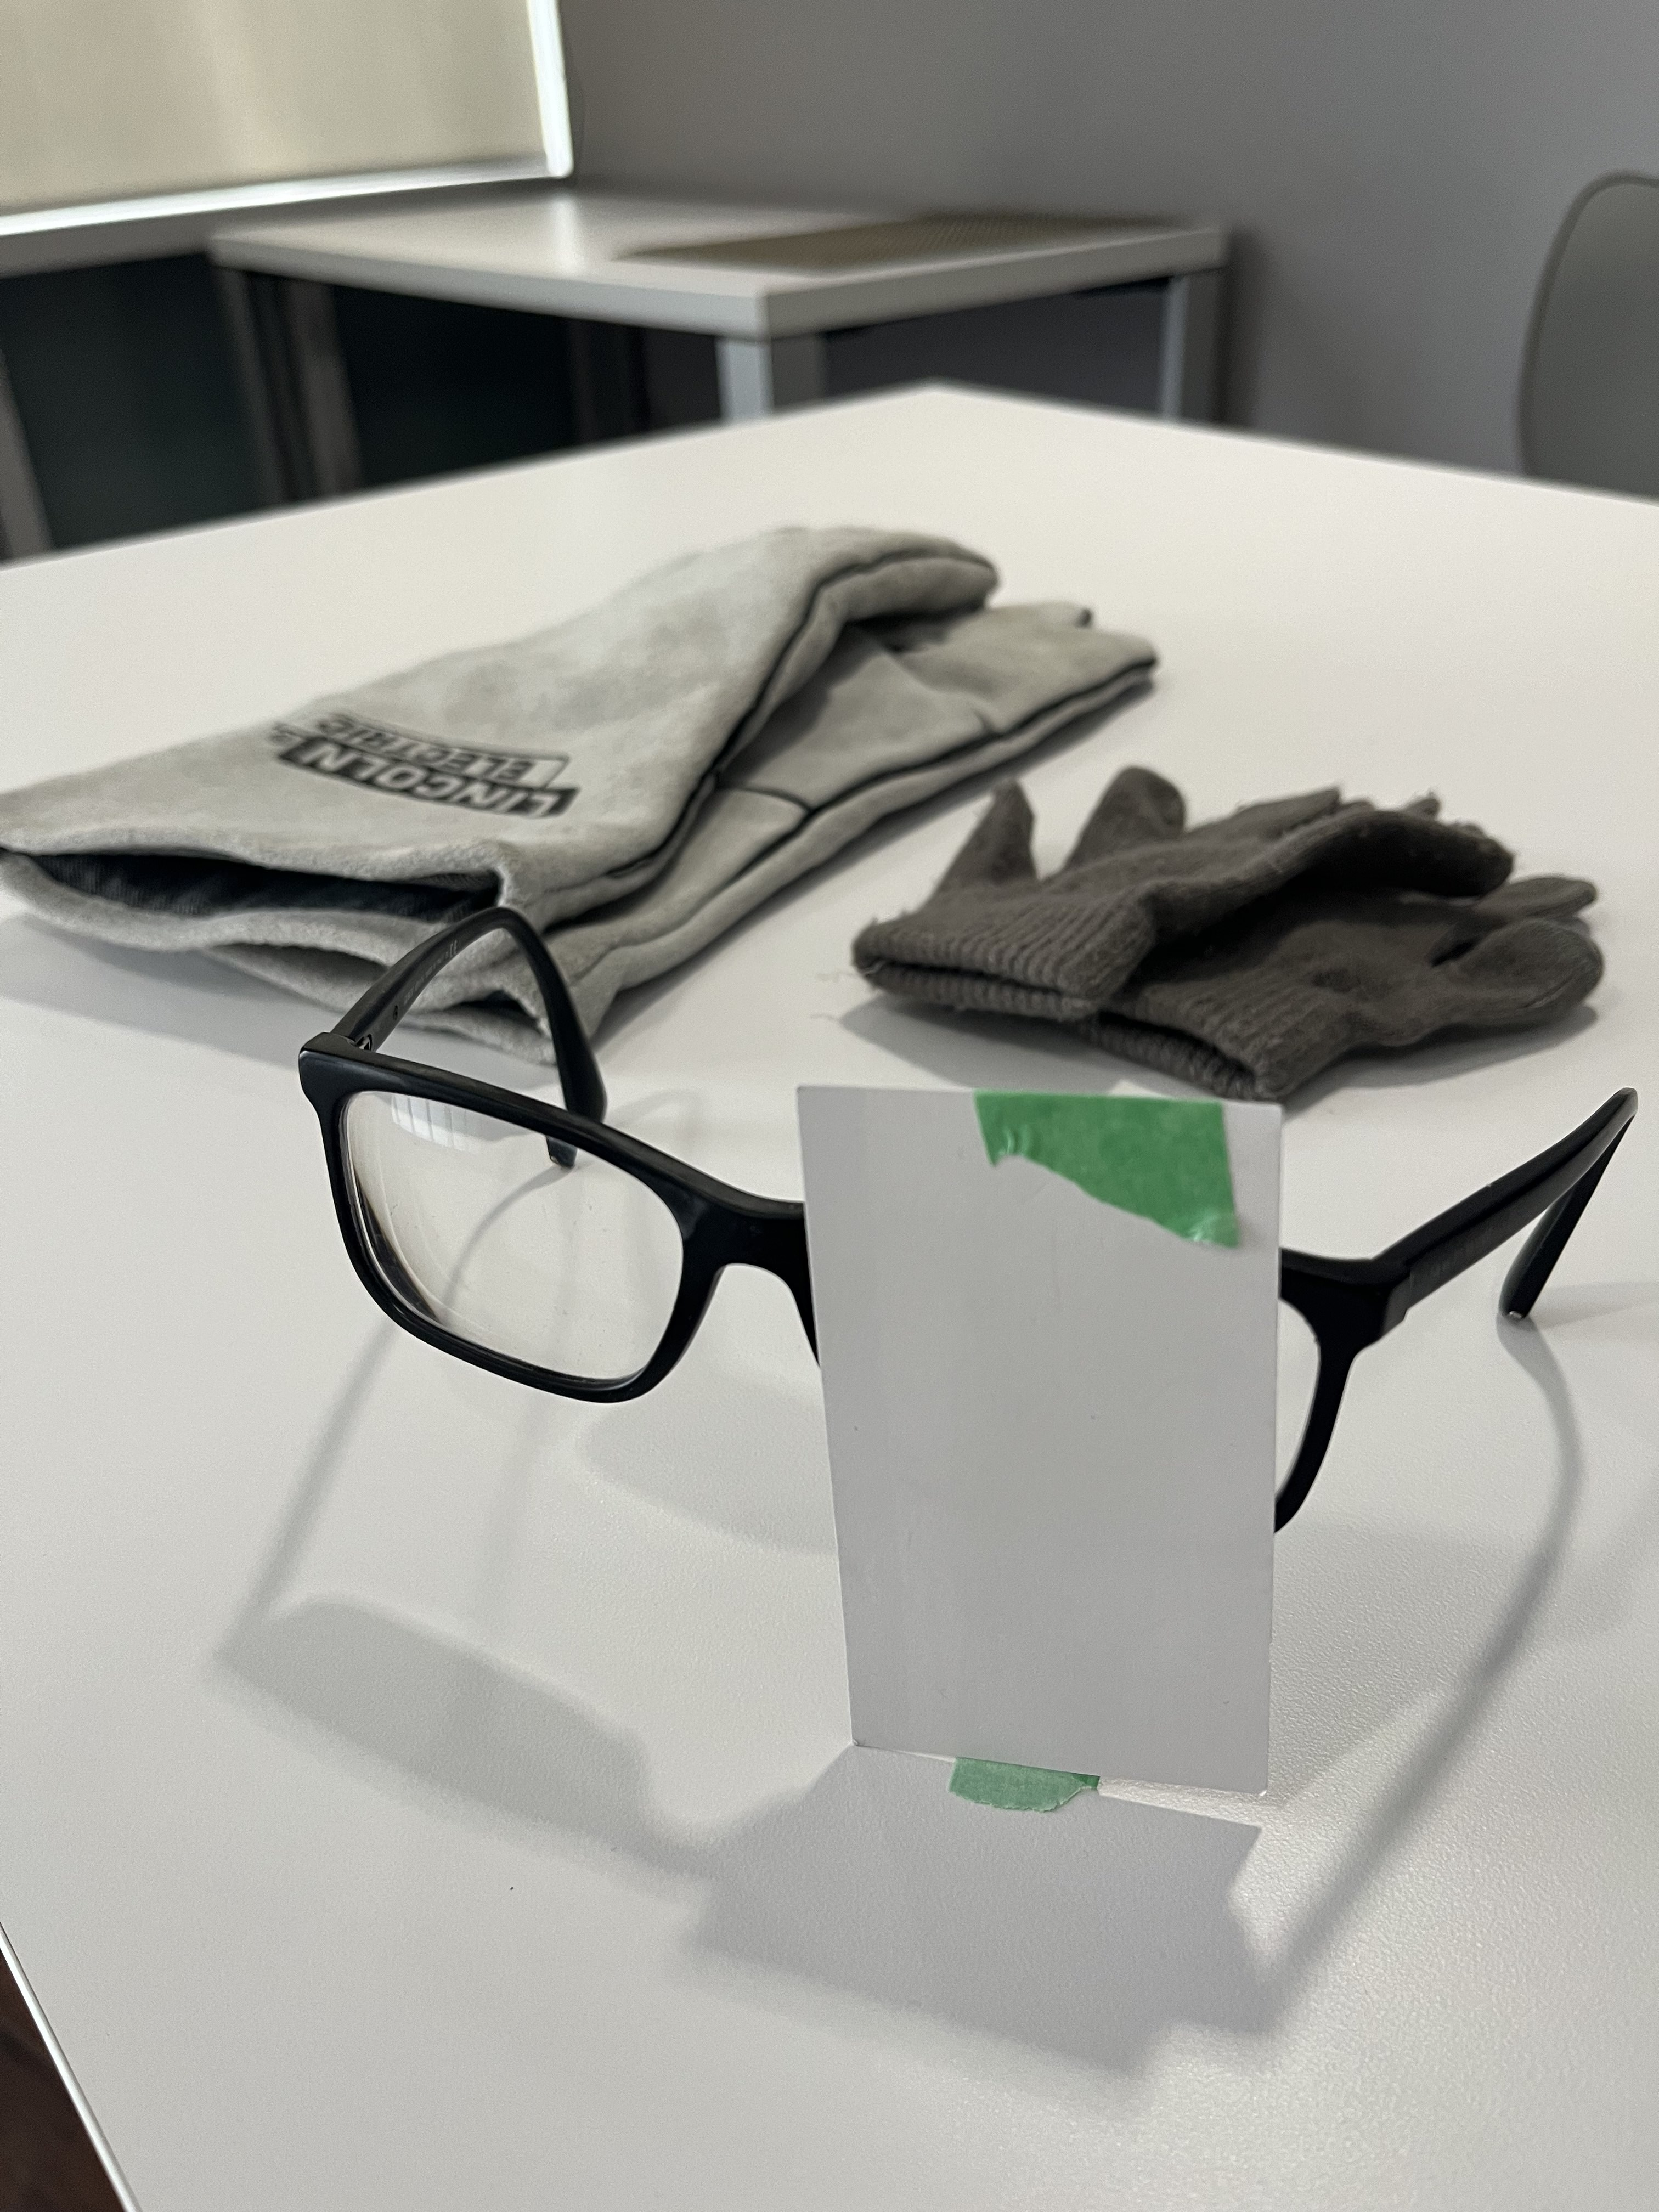
\includegraphics[width=0.6\textwidth]{disability-simulation.jpg}
    \caption{Items used to simulate disability. }
    \label{fig:disability-simulation}
\end{figure}

